\documentclass[12pt]{report}
\usepackage{graphicx}
\usepackage{geometry}
\usepackage[english]{babel}
\usepackage{xcolor}
\usepackage{float}
\usepackage{amssymb}
\usepackage{amsmath}
\usepackage{listings}
\usepackage{color}
\usepackage[utf8]{inputenc}
\usepackage{array}
\usepackage{longtable}
\usepackage{float}
\usepackage[hidelinks]{hyperref}
\usepackage{pgfplots}
\usepackage{fancyhdr}
\pagestyle{fancy}
\graphicspath{{images/}}

\geometry{a4paper, left=2cm, right=2cm, top=3cm}

% remove 'Chapter N'
\usepackage{titlesec}
\titleformat{\chapter}[display]
  {\normalfont\bfseries}{}{0pt}{\Huge}

% bibliography/links
\usepackage[
	backend=biber,
	style=draft,
]{biblatex}
\addbibresource{links.bib}

% custom fields for cover page
\usepackage{titling}
\pretitle{\begin{center}\placetitlepicture\Huge}
\posttitle{\par\lineskip 1em\placesubtitle\end{center}\vskip 3em}
\preauthor{\begin{center}
		\large \lineskip 3em%
		\begin{tabular}[t]{c}}
\postauthor{\end{tabular}\par\placecourse\par\placeprofessor\end{center}}
\predate{\begin{center}\large\vskip 3em}
\postdate{\par\placeversion\par\end{center}}

% commands for including the picture
\newcommand{\titlepicture}[2][]{%
	\renewcommand\placetitlepicture{%
	\includegraphics[#1]{#2}\par\medskip
	}%
}
\newcommand{\placetitlepicture}{} % initialization

% commands for including the subtitle
\newcommand{\subtitle}[2][]{%
	\renewcommand\placesubtitle{%
	\Large #2\par\medskip
	}%
}
\newcommand{\placesubtitle}{} % initialization

% commands for including the course
\newcommand{\course}[2][]{%
	\renewcommand\placecourse{%
	\large Course: #2\par\medskip
	}%
}
\newcommand{\placecourse}{} % initialization

% commands for including the professor
\newcommand{\professor}[2][]{%
	\renewcommand\placeprofessor{%
	\large Professor: #2\par\medskip
	}%
}
\newcommand{\placeprofessor}{} % initialization

% commands for including the version
\newcommand{\version}[2][]{%
	\renewcommand\placeversion{%
	\large Version: #2\par\medskip
	}%
}
\newcommand{\placeversion}{} % initialization

\titlepicture[width=0.75\textwidth]{polimi_logo}
\title{Chatbot Design}
\author{Lorenzo Fratus, 10619073, lorenzo1.fratus@mail.polimi.it \\
Simone Orlando, 10530758, simone.orlando@mail.polimi.it \\
Cristian C. Spagnuolo, 10745353, cristiancarmine.spagnuolo@mail.polimi.it}
\course{Hypermedia Applications}
\professor{Franca Garzotto\\
Delivery date: 28/06/2021\\
Link to prototype: \href{https://securenetwork.herokuapp.com}{securenetwork.herokuapp.com}\\
Github repository: \href{https://github.com/lorenzofratus/SecureNetworkRebrand.git}{SecureNetworkRebrand.git}}


\fancyhead{}
\renewcommand{\headrulewidth}{0pt}
\fancyfoot{}
\fancyfoot[CO,CE]{Lorenzo Fratus, Simone Orlando, Cristian C. Spagnuolo}
\fancyfoot[LE,RO]{\thepage}
\fancypagestyle{plain}{\pagestyle{fancy}}
\begin{document}

\maketitle
\tableofcontents

\chapter{Abstract}
The purpose of this document is to highlight the stages for the 
design of a conversational agent (also referred simply as agent or chatbot) to support 
the users inside the website of the company Secure Network.\\
In particular, we will illustrate the model that describes the process
supported by our chatbot, guiding the reader in understanding each of
the individual states.\\
Finally, we will focus, on one of the possible scenarios, analyzing
it by means of a UML sequence diagram.

\chapter{Model}
This chatbot is designed keeping in mind the two main purposes of the
website:
\begin{itemize}
	\item Advertise the services offered by the company.
	\item Convert the user's visit into a business contact. 
\end{itemize}
\noindent
Figure \ref{fig:model} illustrates the model of this process, the 
meaning of each activity will be better explained in the next chapter.

\begin{figure}[h]
	\centering
	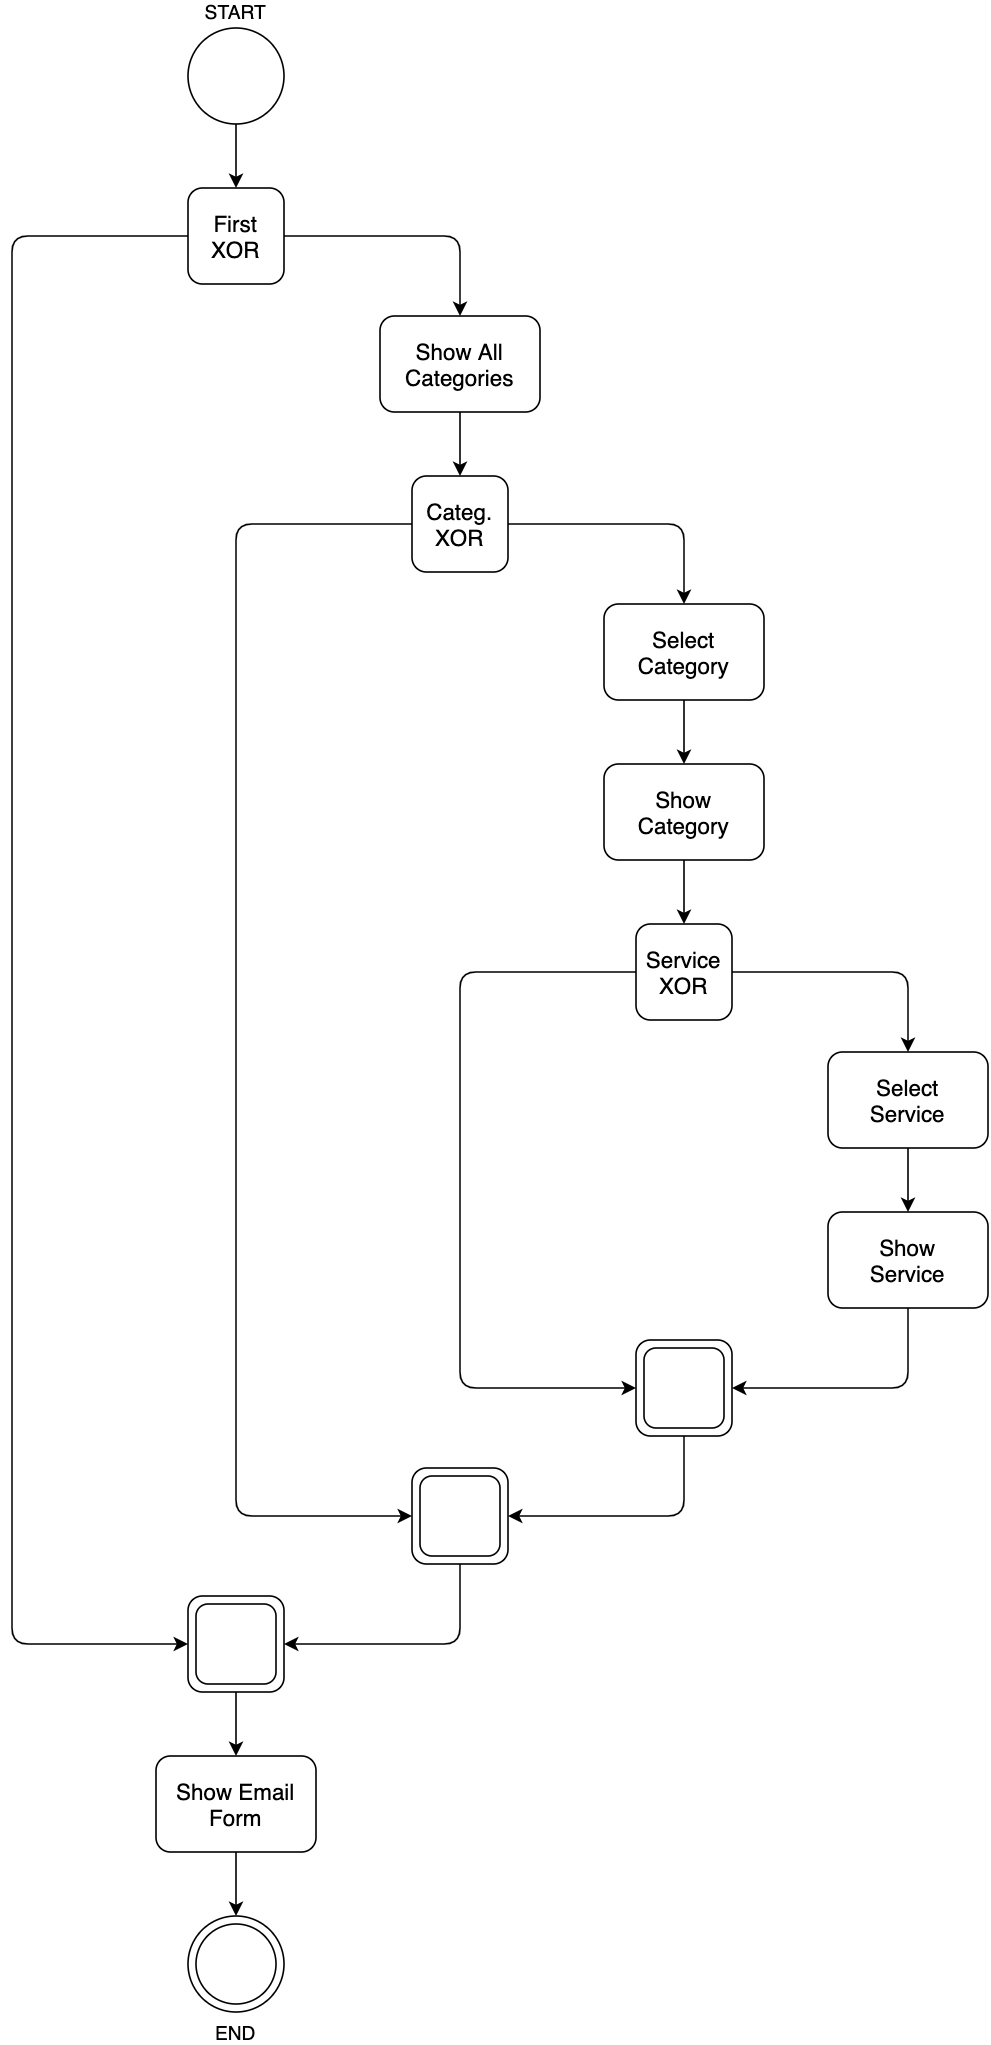
\includegraphics[width=\textwidth]{model}
	\caption{Model of the conversational agent.}
	\label{fig:model}
\end{figure}

\chapter{Activities}
\section{Start \& Exit Activities}
\subsection{Start Activity}
This activity is used as entry point of the interaction, implementing the 
\emph{start} callback. It is used to present the bot to the user and allow to
procede to the next activity without waiting any input by the user. 
No change on the GUI.
\subsection{End Activity}
This activity is used as exit point of the interaction, implementing the 
\emph{exit} callback. It is used to thanks the user for the interaction. 
This activity waits for a new message of the user, in order to re-start the whole 
interaction from the beginning. No change on the GUI.
\section{XOR Activities}
All of the following activities represent exit points strategically placed
within the conversation to convey users to the contact form.
None of them performs direct changes to the GUI. Each of them implements a callback,
which can be called \emph{generic\_xor}, whose goal is to select the right path to take.

\subsection{First XOR}
This is the first activity that is performed during any interaction with
the chatbot. The agent simply greets the user with a short introduction,
after which it asks him if he want to explore the categories of services
offered or if he wants to contact the company.

\subsection{Category XOR}
Here, the chatbot asks the user if he want to continue with the exploration 
of a specific category or if he wants to reach the contact page.

\subsection{Service XOR}
Like the previous ones, this XOR is also an \emph{emergency exit} towards 
the contact page. In this case, the other alternative for the user is to 
take a look at a specific service.

\section{Task Activities}

\subsection{Show All Categories}
The purpose of this task is to move the user's focus to the page containing 
all categories of services. 
The agent interacts with the GUI showing that page, using a callback,
called \emph{nothing}, which contains as a payload a \texttt{guide} field, to
be used for the redirection.
This transition is accompained by a chat message inviting the user to read 
the description of shown categories.

\subsection{Select Category}
Categories shown by the previous task allow the user to procede with this step.
Here, the chatbot asks the user to select the category he want to explore
and awaits his response.
The user can reply in chat, with the name of the category or directly click on one 
of the buttons in the GUI, which will fill the chat for the user.
No change on the GUI happens during this task. Again, the \emph{nothing} callback can 
be used, this time with an empty payload.

\subsection{Show Category}
This is also a transitional activity, the chatbot interacts with the GUI to 
bring the user to the page of the chosen category, using the \emph{nothing} callback, 
with the proper payload. As always, a chat message tells the user to read the description 
of presented services.

\subsection{Select Service}
This is the beginning of the deepest nesting level of this conversation.
The agent asks and waits for the name of a specific service belonging to the 
category that the user has selected in the previous steps.
Even in this case, the user can reply by pressing the button of the specific
service. No changes in the GUI. The \emph{nothing} callback with empty payload
is used.

\subsection{Show Service}
After the selection, the agent opens the page containing the description of 
that specific service, using the \emph{nothing} callback, with the proper payload.
As usual, the agent displays a message in chat but in this case also waits 
for user input before continuing with the process.
\clearpage
\subsection{Show Email Form}
This is the final point of confluence of any conversation.
Here, the agent will take the user directly to the contact page, more
precisely at the section containing the contact form, again, using the \emph{nothing} callback, 
with the proper payload.
The chatbot will use the \texttt{subject} field of the payload 
to pre-fill, the \emph{Subject} field of the form,
as well as a short introductory sentence in the \emph{Message}, based
on the knowledge acquired during the previous interaction, passed through the \texttt{intro} field of the payload.
After the user has sent the message, the conversation will end with a farewell phrase.

\chapter{Scenario}
\emph{Antonio} is a 43 years old Italian entrepreneur. 
He is the head of a medium-sized logistics company in the hearth of Lodi and would like to hire Secure Network to make sure his IT infrastructure has no vulnerabilities.
\emph{Antonio} is not a PC expert and usually appreciates help while navigating, so he heads straight to the website chat.

In Figure \ref{fig:sequence-diagram} is shown his interaction with the conversational agent.
Note that, for the sake of brevity, the messages between the chatbot and the user have been limited to the bare minimum.

\begin{figure}[h]
	\centering
	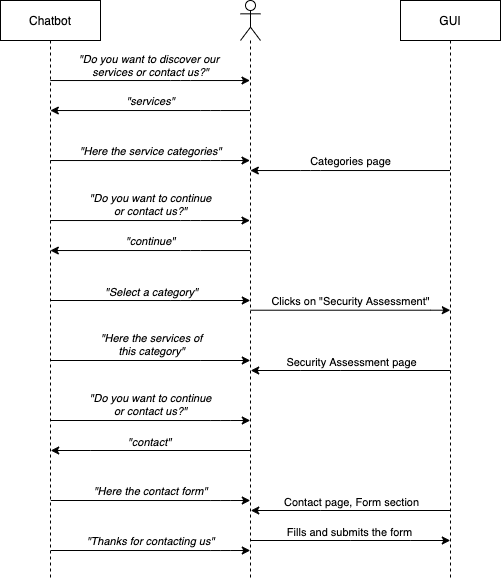
\includegraphics[width=\textwidth]{sequence-diagram}
	\caption{Sequence diagram of an interaction example.}
	\label{fig:sequence-diagram}
\end{figure}

\chapter{ChatBot Implementation} 
To complete the second part of the chat bot optional project, we followed the documentation available at Multi Modal Chatbot Creator (https://gitlab.com/i3lab/mmcc/frontend/mmcc-vue/-/blob/master/README.md).
At the beginning, the user is asked whether he wants explore the website or he wants to contact the company. 
If the user wants to explore the website, the chatbot first introduce itself, then it shows the home and the about page of the website.
If the user wants to contact the company, the chatbot asks whether the user want to fulfill a form or go to the contact page. In either case, 
it redirects the user to the correct page. The configuration file used for the integration of the chatbot can be found at ./chatbot/config/chat-bot.json and reflect the model provided by the assignment specification.
At the current state of the art of the provided backend of the Multi Modal Chatbot Creator, there is no native way of performing a loop upon reaching the end activity, even if the next\_id field of the 
end task is set to a previous activity. Moreover, upon reaching the terminal state, the user will receive the same terminal answer for each additional message sent. We have already informed developers which 
will provide in the next versione a reset callbat to support such this behaviour. To follow the exact model provided by specification, we didn't apply any custom patch.


\end{document}